\section{The induced mean current: Dysthe's central new effect}
\label{sec:mean}
\subsection{Averaging reveals a response invisible in the carrier alone}
Quadratic wave quantities such as velocity products have a nonzero
carrier-period average. The wave therefore carries averaged momentum flux.
The wave contribution to that flux is called \emph{radiation stress}.
Here radiation means transport by waves, not electromagnetic radiation.
A uniform flux has no horizontal divergence; a spatially modulated flux
can exert an averaged force and generate a mean-flow response.

This is a physical interpretation. Dysthe determines the mean response
from the averaged potential-flow surface conditions, not by introducing
a separate viscous forcing law. The induced current remains irrotational
under the paper's hypotheses.

In dimensional variables his (2.9)--(2.11) read
\begin{align*}
 \Ph_t+g\Zh&=0,&&z=0,\\
 \Ph_z-\Zh_t&=\frac{2\omega_0}{g}\boldsymbol{k}_0\cdot
                   \nabla_h|A_{\rm dim}|^2,&&z=0,\\
 \nabla^2\Ph&=0,&&z<0.
\end{align*}
The dimensions of the forcing and of $\Ph_z$ are both velocity.
In carrier-scaled variables, these become
\begin{equation}\label{eq:mean-full}
 \Ph_t+2\Zh=0,\qquad
 \Ph_z-2\Zh_t=\partial_x|A|^2,\qquad
 \nabla^2\Ph=0.
\end{equation}
The first equation gives $\Zh=O(\varepsilon^3)$ because
$\Ph=O(\varepsilon^2)$ and its time derivative is slow.
Thus $\Zh_t=O(\varepsilon^4)$, whereas $\Ph_z$ and
$\partial_x|A|^2$ are third order. At the retained order,
\begin{equation}\label{eq:mean-bc}
 \Ph_z=\partial_x|A|^2\quad(z=0),\qquad
 \nabla^2\Ph=0\quad(z<0).
\end{equation}
Together with decay at depth and a choice of zero background current,
this determines the mean velocity. An additive potential constant is a
gauge freedom and has no physical velocity.

\subsection{Solve the boundary problem one Fourier mode at a time}
Let $I=|A|^2$, and suppose it has a Fourier component
$\widehat I e^{i(\lambda x+\mu y)}$ with
$K=\sqrt{\lambda^2+\mu^2}>0$. Seeking a decaying solution gives
\[
 \Ph=C e^{Kz}e^{i(\lambda x+\mu y)}.
\]
The surface condition is $KC=i\lambda\widehat I$, so
\begin{equation}\label{eq:mean-symbol}
 \widehat{\Ph}(0)=\frac{i\lambda}{K}\widehat I,
 \qquad
 \boxed{\widehat{\Ph_x}(0)=-\frac{\lambda^2}{K}\widehat I.}
\end{equation}
The horizontal current has a negative real Fourier multiplier. This is
exactly the source of the $\lambda^2/K$ term in the stability result.

At $K=0$, the forcing is zero. Set the derivative response to zero;
do not divide by $K$. A uniform wavetrain generates no mean-current
\emph{forcing in this model}. This does not mean that water under a
uniform Stokes wave has no particle drift. Eulerian induced mean flow and
Lagrangian Stokes drift are different quantities.

\subsection{Nonlocality and the Hilbert transform}
With no $y$ dependence, $K=|\lambda|$ and the current multiplier is
$-|\lambda|$. Define $|D_x|$ by the Fourier multiplier $|\lambda|$.
For the transform convention
\[
 \widehat f(\lambda)=\int_{\RR}f(x)e^{-i\lambda x}\,\rad x,
\]
the Hilbert transform $H$ has multiplier $-i\operatorname{sgn}\lambda$,
so $H\partial_x=|D_x|$. Consequently
\begin{equation}\label{eq:hilbert}
 \Ph_x(x,0)=-|D_x|I(x)=-H\partial_x I(x).
\end{equation}
This is nonlocal: knowing intensity at one point is not sufficient to
calculate the current there. One must solve the half-space problem, or
apply its Fourier multiplier to the full profile. Periodic profiles use
the corresponding discrete multiplier and zero mode.

\begin{example}[An explicitly solvable intensity modulation]
Let $I(x)=I_0+I_1\cos(\kappa x)$, where $\kappa>0$ and
$|I_1|<I_0$. Then
\[
 \Ph=-I_1e^{\kappa z}\sin(\kappa x),\qquad
 \Ph_x(x,0)=-\kappa I_1\cos(\kappa x).
\]
Differentiate to verify both Laplace's equation and
$\Ph_z=I_x$ at $z=0$. For $I_1>0$, the current response at an intensity
maximum is opposite the carrier propagation direction under this convention.
The response penetrates depth $1/\kappa$.
\end{example}

\begin{figure}[htbp]
\centering
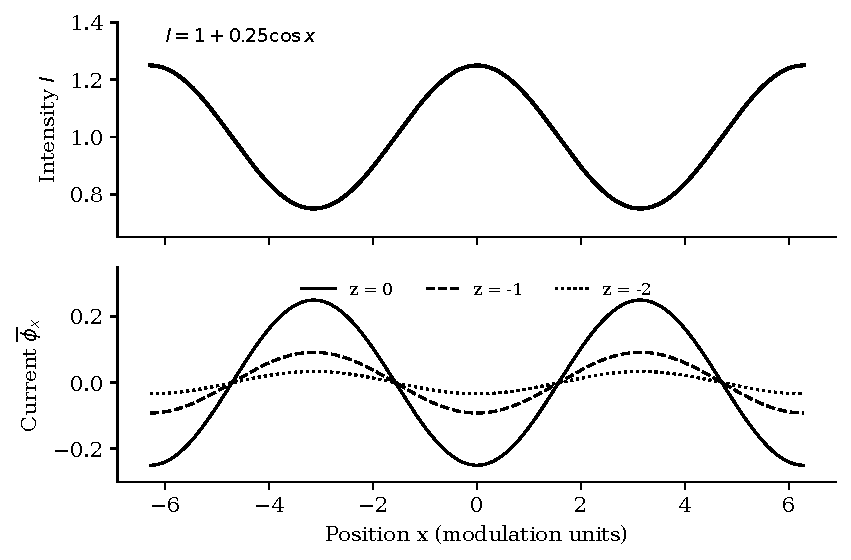
\includegraphics[width=.90\linewidth]{figures/mean-flow.pdf}
\caption{The cosine intensity example. The mean horizontal current
$\Ph_x$ is in opposite phase to the intensity variation, and its amplitude
decays as $e^{\kappa z}$. Vertical profiles use illustrative values;
the curves depict the analytic half-space solution.}\label{fig:mean}
\end{figure}

\subsection{Why a small current affects wave stability}
For a weak, slowly varying along-wave current $U$, the local dimensional
frequency has a Doppler contribution $k_0U$. In Dysthe's scaled envelope
equation the current is represented by $A\Ph_x$. Because the physical
scaling gives $k_0U/\omega_0=\Ph_x/2$, a locally uniform current produces
the expected envelope phase shift after the factor $2i$ is accounted for.

The intensity changes the current, the current changes local phase, and
phase changes feed back on the modulation. It is a coupled stability
mechanism. Calling it detuning does not imply that every disturbance is
stabilized or that the wave loses energy to viscosity.

\paperlink{Read (2.9)--(2.11), (2.20)--(2.21), and (4.1)--(4.3).
Then read the four physical steps on printed p.~114.}
\checkpoint{Derive the multiplier $-\lambda^2/K$ without using a
Hilbert-transform identity.}
\clearpage
